\documentclass{article}
\usepackage{../../../settings}

\begin{document}
\hexcover{APCS 從零到三級跳}{學習歷程}{作者：曾嘉禾}{Tan}{2025}

\begin{large}

\begin{boxpar}{Tan}{製作動機}
加入電算社後接觸了更多程式設計的應用場景，但我意識到自己的演算法基礎幾乎是空白的。在日常開發中我能把功能寫出來，卻無法分析程式的效能邊界，遇到複雜題目只能靠直覺猜解法。因此決定以 APCS 檢定作為目標，透過系統性的練習補足這塊缺口，並驗證自己的程式實力。
\end{boxpar}

\begin{boxpar}{Tan}{自學歷程}
準備期間主要透過線上題庫（ZeroJudge）與演算法筆記自學，沒有使用補習班或課程。從最基礎的陣列操作與迴圈邏輯開始，逐步推進到排序、搜尋、遞迴與動態規劃。過程中最大的挑戰不是記住演算法本身，而是學會在看到題目的第一秒判斷應該套用哪種策略。這種題型識別的能力只能靠大量練習積累，沒有捷徑。

練習檔案紀錄（C 與 C++ 共計逾 240 份）：

\begin{itemize}
    \item C 語言：基礎資料結構與邏輯題
    \item C++：進階演算法與 APCS 歷屆試題
\end{itemize}
\end{boxpar}

\begin{boxpar}{Tan}{成績證明}
    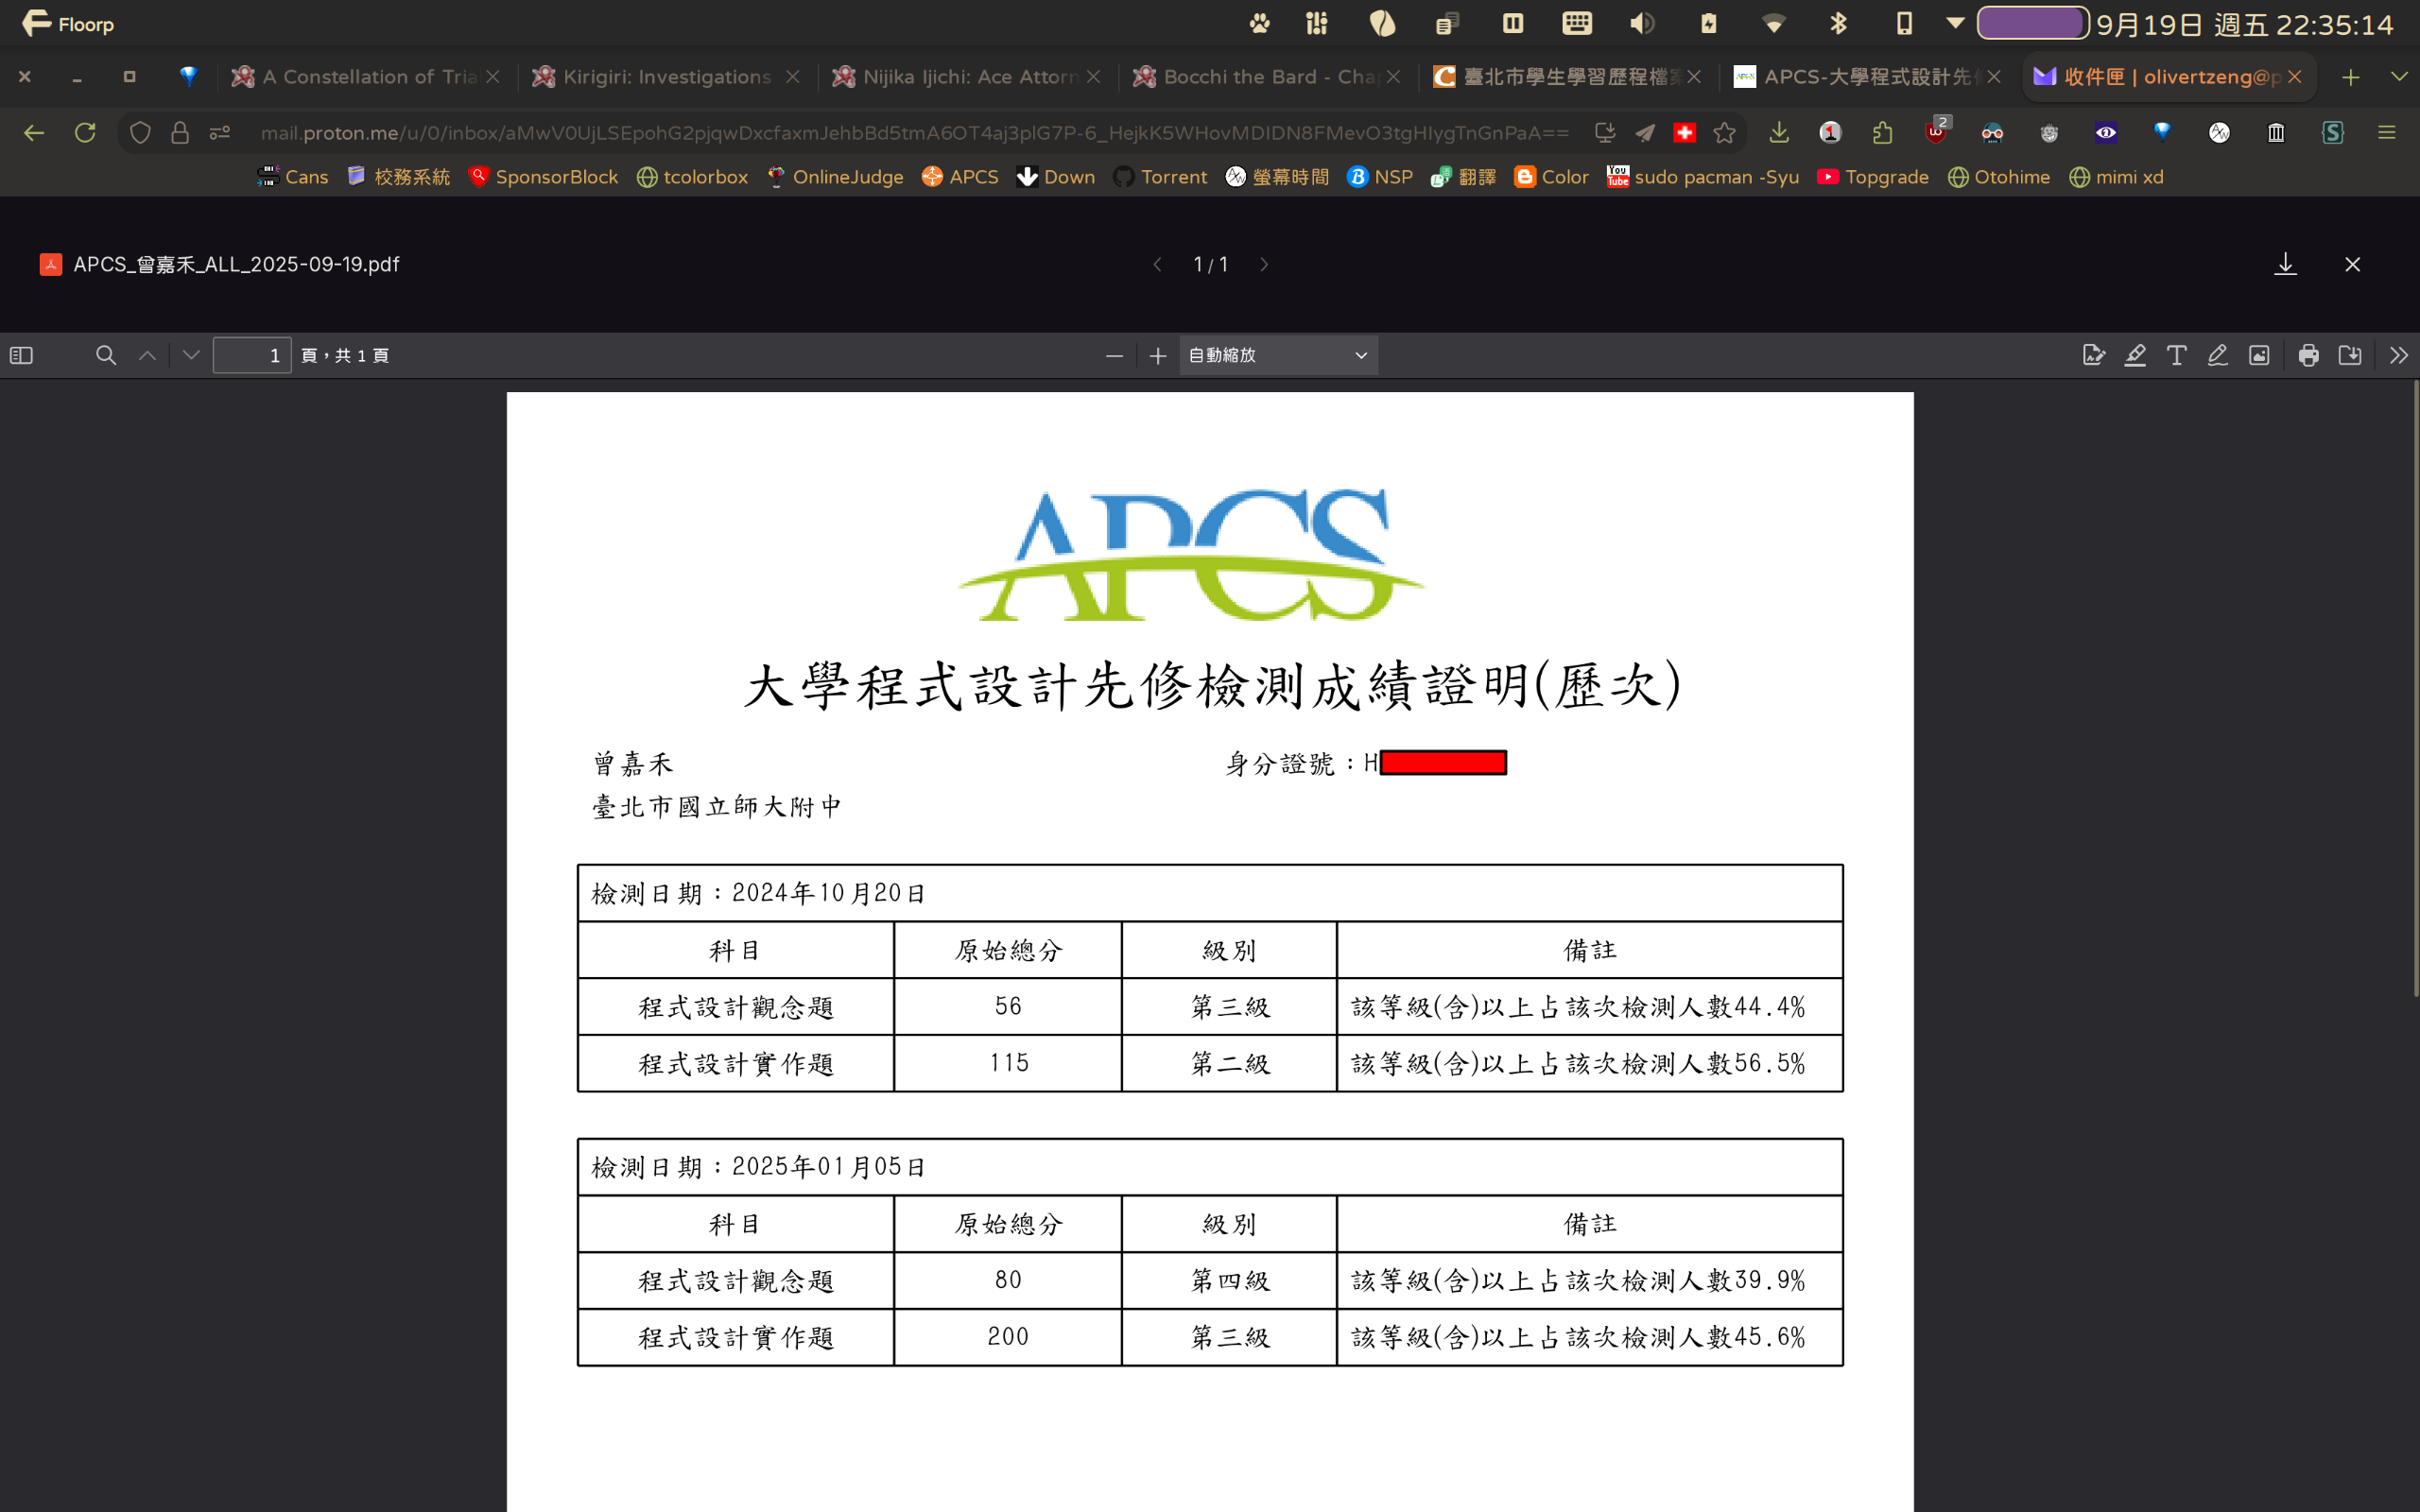
\includegraphics[width=\linewidth]{src/proof.png}
\end{boxpar}

\begin{boxpar}{Tan}{反思}
通過觀念題四級與實作題三級後，我意識到這個成績代表的不只是「會寫程式」，而是開始能用演算法語言思考問題。但同時也更清楚地看見自己的上限。實作題三級與四級的差距，在於能否在時間壓力下快速建構出正確的資料結構組合。這個能力需要更深的數學基礎與更多的訓練以建立起實戰的經驗。
\end{boxpar}

\begin{boxpar}{Tan}{未來展望}
這次準備 APCS 讓我確認了一件事。演算法能力是工程師的底層語言，不是可以靠直覺繞過去的東西。往後不管投入哪個開發領域，能夠分析程式的時間與空間複雜度，會是讓作品從「能動」變成「穩定」的關鍵能力。
\end{boxpar}

\end{large}
\end{document}
